\documentclass{sig-alternate}

\usepackage{cite}
\usepackage{url}
\usepackage{color}
\usepackage{listings} % Used for showing code
\usepackage{wrapfig}
\usepackage{multirow}

% See which ones of these we can get rid of
%\usepackage{colortbl}
%\usepackage{graphicx}
%\usepackage{blindtext}
%\usepackage{multicol}


\newcommand{\todo}[1]{\textcolor{cyan}{\textbf{[#1]}}}
\newcommand{\wei}[1]{\textcolor{green}{{\it [Wei says: #1]}}}
\newcommand{\dan}[1]{\textcolor{blue}{{\it [Dan says: #1]}}}

\lstset{
  language=C,
  basicstyle=\small,
  breaklines=true
  }



\begin{document}

\conferenceinfo{MSR}{'14 Hyderabad, India}

\title{A Code Clone Oracle}

\numberofauthors{1}
\author{
%
%
\alignauthor
Daniel E. Krutz and Wei Le\\ 	
	\affaddr{Software Engineering Department}\\
       \affaddr{Rochester Institute of Technology, USA}\\
       \affaddr{1 Lomb Memorial Drive}\\
       \affaddr{Rochester, NY 14623} \\
       \email{\{dxkvse,wei.le\}@rit.edu}
}

 % Must not be a space above this

\maketitle
\begin{abstract}

Code clones are functionally equivalent code segments. Identifying code clones is very important for determining bugs, fixes and software reuse. Code clone detection is also essential for developing fast and precise code search techniques.\dan{I am a bit confused by this sentence, maybe reword it} However, the challenge of such research is to evaluate that the clones detected are actually functionally equivalent, considering the majority of clones are not textual or even syntactically identical. In fact, we found that different tools report inconsistent results regarding what is a clone. The goal of this work is to generate a set of high-confident code clones to help future code clone detection and code search tools to evaluate their techniques. We studied three open source programs, {\it Apache}, {\it Python} and {\it PostgreSQL}, and randomly sampled a total of 1536 function pairs. We first applied multiple code clone detection tools to identify code clones. Meanwhile, we built a tool to automatically load function pairs of interest and record the manual inspection results on whether or not the two functions are clones. We recruited three {\it experts} who have experience in clone detection research and four students who have experience in programming to manually determine code clones and their types. We found 66 pairs of clone functions that agreed by both tools and human inspection results, which can be used as an oracle for future researchers to determine whether a tool successfully identified code clones and their types. The 66 pairs cover all 4 types of clones. Interestingly, only 1 pair is {\it type 1}, which is textual identical, and 9 pairs are {\it type 4} clones, which only can be determined by comparing input and output of the functions.


\end{abstract}

%\todo{Update}
% A category with the (minimum) three required fields
%\category{H.4}{Information Systems Applications}{Miscellaneous}
%A category including the fourth, optional field follows...
%\category{D.2.8}{Software Engineering}{Metrics}[complexity measures, performance measures]

%\terms{Theory}

%\keywords{ACM proceedings, \LaTeX, text tagging}



\section{Introduction}

% Use Information from the Lavoie paper to help discuss why the creation of a good oracle is so important. It has some good information in the introduction section of the paper.

Code clones are multiple fragments of source code that may be syntactically different, but are functionally equivalent. Code clones may adversely affect software in a variety of ways. Some of which include elevating the maintenance costs of a project, since the same alterations may need to be done several times, and inconsistent bug fixes leading to increased system faults~\cite{Roy:2009:CEC:1530898.1531101}.

% Probably change up this paragraph a bit
Clones have been classified into four primary groups. Type-1 clones are the simplest and represent identical code except for variations in whitespace, comments and layout. Type-2 clones are syntactically equivalent except for differences in identifiers and types. Type-3 clones are two segments which differ due to altered or removed statements. Type-4 clones are the most difficult to detect and represent two code segments which considerably vary syntactically but produce identical results when executed~\cite{Roy:2009:CEC:1530898.1531101}.

Numerous tools and techniques have been proposed to discover code clones using a variety of different and highly effective methods~\cite{Roy:2009:CEC:1530898.1531101}. When measuring the effectiveness of new or existing tools in terms of precision, recall, or in their ability to discover different types of clones, they are often evaluated against clone oracles~\cite{Kim:2011:MMC:1985793.1985835, Lavoie:2011:ATC:1985404.1985411}. These oracles are usually small classes, containing only 5-20 known clones, with the tools being evaluated on how well they can find the known clones and not identify false positives~\cite{Kraw2012}.

Some oracles are created exclusively by manually analyzing applications for clones. This is a difficult and time consuming task since it is very hard to manually identify more complicated varieties of clones, such as type-4 clones. Additionally, manually identifying clones is a difficult and imprecise task even for researchers very experienced with clone detection~\cite{Walenstein:2003:PCT:950792.951349}. In other instances, oracles are created through the use of a single clone detection tool, which creates a bias towards the tool and the clones it is able to find.

In the following work, we present a publicly available code clone oracle which is substantially sized, and has been generated through a mixture of manual analysis and several leading clone detection tools. To create this oracle, we first selected several well known open source applications and had researchers and students independently examine them for clones. Next, several leading clone detection tools were run on this code base. The results from these tools were mixed with the findings from the manual analysis phase to determine the clones in each system, in addition to the type of clone found. A separate student group also provided a separate rating of the clone pairs.

This paper is innovative because there are no known existing clone oracles which are substantially sized, we explicitly define all four types of clones, and the oracle has been created through a mixture of manual verification and several leading clone detection tools to eliminate as much potential bias as reasonably possible.

The rest of the paper is organized as follows. Section~\ref{sec: oraclecreation} describes how the oracle was created and some of the contents from the oracle including the amount of each type of clone discovered and how many functions in each application were not clones. Section~\ref{sec: relatedworks} provides an overview of related works, while Section~\ref{sec: futurework} discusses future work to be done on this area. Finally, Section~\ref{sec: conclusion} provides concluding remarks to this work.


\section{Oracle Creation} % How was the oracle created
\label{sec: oraclecreation}

In the following sections, we describe our selection of the source code of several applications, and our identification of code clone candidates through the use of manual analysis and with the assistance of several leading clone detection tools. We also discuss how our data is made available to other researchers for use in their own work.

\subsection{Clone Identification}
The initial step in the oracle creation process was to select several existing applications to examine for clones. We chose Apache 2.2.14\footnote{http://www.apache.org}, Python 2.5.1\footnote{http://www.python.org} and PostgreSQL 8.5\footnote{http://www.postgresql.org} since they are significantly sized, well known applications which have already been used in previous clone detection research~\cite{Kim:2011:MMC:1985793.1985835}. These were analyzed as-is and had no alterations performed to their source code. For this analysis, we decided to search for clones at the method level. This precision was chosen since manually analyzing code at a more fine-grain level would not have been reasonably possible due to the immense amount of manual effort required by this task. The examined source code is available on the project website.

Two separate groups manually analyzed the possible clone pairs. One was three researchers very familiar with code clones, which we will refer to as our clone experts, and four students who also analyzed the candidate clone pairs. While the expert group discussed their findings to come to a consensus, we merely report the percentage of students who identified if a candidate pair represented a clone. The results from the two groups are shown independently of each other. Our goal for having these two groups was to present more information for future researchers to consider, and use if they should desire. A secondary goal was to see how much the findings of the expert and student groups differed from one another.
% Leave this part in about secondary goals? This needs to be discussed then?

The four types of clones as defined by Roy~\emph{et al.}~\cite{Roy:2009:CEC:1530898.1531101} were used as guidance in identifying and classifying clones. In order to manually evaluate each of the systems for clones at the method level, all methods in the application would need to be compared against all other methods in the application in a round robin fashion, with the clones and their types being recorded. The number of comparisons done using this process was extremely large, as show in Formula~\ref{eq:roundrobin}, so even an application with 100 methods would need to have 4,950 comparisons performed.

\begin{equation} \label{eq:roundrobin}
(Method Count *(MethodCount-1))/2
\end{equation}

%(100 *(99))/2
%(fileinfolist.size()*(fileinfolist.size()-1))/2;

To make this process more manageable, we randomly chose a small subset of 3-6 class files from each application to examine for clones. We arbitrarily selected several classes in each application for analysis, with the only selection criteria being that each class was to contain at least ten methods so that we would have an adequate number clone candidates. The number of possible clones in these subsets for the three applications was still over 45,000; which is not reasonable to check for through manual analysis. To make this number more manageable, we randomly selected a statistically significant number of clone possibilities to examine with the goal of having a confidence level of 99\% and a confidence interval of 5.

%We also ignored methods that were under 3 lines long which eliminated

% In order to be considered a clone, candidates had to be at least three lines long. - Should I leave this?

We developed an open source tool known as~\emph{GraphicDiff}~\footnote{https://code.google.com/p/dek-graphicdiff/} to assist with the manual clone identification process. This tool automatically displayed each of the methods to be compared and allowed the user to select if the comparison represented a clone, and if so what type. Once the user was finished examining a candidate clone pair, they could then easily cycle onto the next candidate pair. Each research group independently examined the applications using GraphicDiff, with their findings recorded. GraphicDiff is represented in Figure~\ref{fig:graphicdiff}. % Provide screenshot of this tool?

% postgre 25769
\begin{figure}[ht!]
\centering
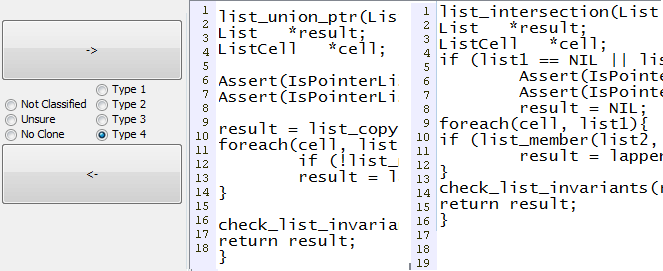
\includegraphics[width=83mm,height=43mm]{images/gd5.png}
\caption{GraphicDiff}
\label{fig:graphicdiff}
\end{figure}

\subsection{Expert Group}

The clone identification process for our expert group was assisted by several leading clone detection tools including Simcad\cite{6613857}, Nicad\cite{Roy:2008:NAD:1437898.1438600}, MeCC\cite{Kim:2011:MMC:1985793.1985835} and CCCD~\cite{wcre2013}. The results of each clone comparison for all of the tools were recorded. This step was done after manual analysis in order to eliminate any possible influence on the initial manual analysis phase.

There were numerous discrepancies between the evaluators during the manual analysis phase. In order to help mitigate these disagreements as to whether or not two methods were clones, or even what type of clone they represented, results from the various tools were used by the researchers to assist with the decision making process. Using these results as input, discrepancies were discussed until an agreement could be made. There were cases however, where no agreement could be made with these results being recorded as~\emph{unsure} in the final result set.

If several of the clone detection tools indicated a clone, where none was noted during manual analysis, the reviewers re-evaluated the candidate clone pair to ensure they had not overlooked anything. The same process was used in reverse when the tools indicated no clone, but manual analysis had found a clone pair. Ultimately, the final decision on a possible clone pair was made by the researchers, and not by any tool.

\subsection{Student Group}
A group of four students examined the same set of candidate clone pairs as the expert group to provide a larger, more diverse set of results for consideration. All  were upper division software engineering students who had no prior experience with code clones. To help familiarize students with code clones, they were asked to read papers by Roy~\emph{et al.}~\cite{Roy:2009:CEC:1530898.1531101}, Kim~\emph{et al.}~\cite{Kim:2011:MMC:1985793.1985835}, and Lavoie and Merlo~\cite{Lavoie:2011:ATC:1985404.1985411}. Finally, all students were independently interviewed to ensure that they understood code clones at an acceptable level.

The students did not discuss their results or come to a conclusion with other student examiners, and were not provided with any results from clone detection tools, or from the expert group. For each candidate clone pair, the percentage of students who identified it as a clone are presented for use at the discretion of the researcher. Like the expert group, the students used GraphicDiff to assist in the clone identification process.

\subsection{Results}
Our created oracle is available on our project website\footnote{\url{http://www.se.rit.edu/~dkrutz/cloneoracle/}} in several formats including html, csv, xml and xls. Table~\ref{table:exampleoutput} shows an example set of publicly available data. The comparison column lists the two methods which were evaluated. The expert column displays the type of clone agreed upon, and a "No" if a clone was not found. The student column shows the percentage of students who found the pair to represent a clone. Finally, subsequent columns list the tools used as part of the analysis and if they found the pair to represent a clone. Since only a subset of comparisons were manually examined by either of the two human groups, the comparisons which were not manually analyzed were left blank.

\begin{table}[thb!]
\begin{center}
\caption{Example Results Output}
\label{table:exampleoutput}
    \begin{tabular}{ l | l | l | l | l  }
%    \toprule
   \bfseries Comparison &\bfseries Expert & \bfseries Student & \bfseries Tool 1 & \bfseries Tool 2 \\ \hline \hline
   \bfseries MethA-MethB  & Type 1 & 100 & No   & Yes  \\ \hline
\bfseries MethB-MethC &  &  & No   & No  \\ \hline
\bfseries MethA-MethB & Type 3 &  75  & Yes   & Yes   \\ \hline
\bfseries MethD-MethE & No &  0  & No   & No   \\

    \end{tabular}
\end{center}

%\vspace{-0.3in}
\end{table}


Table~\ref{table:clonesfound} displays the various types of classifications as noted by our~\emph{expert} and~\emph{student} groups. The clones were broken down by type for the expert group, while the student group was not since they were only asked to identify the clones, not classify them. The relatively small number of type-4 clones identified in the oracle is because even the best clone detection tools struggle at finding these most complicated types of clones and identifying them through manual analysis is a very difficult task due to their complexity~\cite{Roy:2009:CEC:1530898.1531101}. No type-1 clones were noted, which is not surprising since developers can usually recognize exact duplications of code and would have removed them from the software. All of the type-4 clones were initially manually classified as type-3 clones. Only after a subsequent discussion among the researchers did they conclude that they were actually type-4 clones.

\dan{I left the section about total clones found by 50\% of the student researchers. Feel free to remove it.}

The number of clones discovered for each group of evaluators significantly differed. While there were only 5 more clones identified by the student group in Apache, this number grew to 19 in Python and 74 in PostgreSQL. There are several reasons for these variations. The first is that we only used 50\% as the identification criteria for the student group and reducing this value would have removed many of the clones identified by the students. However, we wanted to present these findings for future researchers to use at their discretion and therefore decided to keep the classification criteria at 50\%. Additionally, there is expected to be a large amount of variation for the manual classification of clones, so a significant about of deviation is expected~\cite{Walenstein:2003:PCT:950792.951349}. The~\emph{Agree} column is the number of clones identified by the expert group, that were identified as clones by at least 50\% of the student group. The students agreed with the majority of clones in Python and P-SQL, but only 7 of the 18 clones in Apache.

\dan{Should we attempt to explain why? I don't really have a firm reason.}

\begin{table}[thb!]
\begin{center}
\caption{Clones Identified in Oracle}
\vspace{0.1in} % Add a small buffer between title and table
\label{table:clonesfound}
\begin{tabular}{r||l|l|l|l}
%  \hline
\bfseries Application & \bfseries Clone & \bfseries Expert & \bfseries Student & \bfseries Agree \\ \hline\hline
  \bfseries Apache & \bfseries  T1 & 0 &  \\ \cline{2-3}
   & \bfseries T2 &  18 & \\ \cline{2-3}
& \bfseries  T3 &  0 &  \\ \cline{2-3}
& \bfseries  T4 &  0 &  \\ \cline{2-5}
& \bfseries Total &  18 & 23 & 7 \\ \cline{2-5}
& \bfseries Not Clone &  339 & 334 & 303 \\ \cline{2-5}

\hline
  \bfseries Python & \bfseries T1 & 0 &  \\ \cline{2-3}
   & \bfseries T2 &  7 & \\ \cline{2-3}
& \bfseries  T3 &  4 &  \\ \cline{2-3}
& \bfseries  T4 &  4 &  \\ \cline{2-5}
& \bfseries Total &  15 & 34 & 12 \\ \cline{2-5}
& \bfseries Not Clone &  530 & 522 & 473 \\ \cline{2-5}
\hline

  \bfseries P-SQL & \bfseries T1 & 0 &  \\ \cline{2-3}
   & \bfseries T2 &  18 & \\ \cline{2-3}
& \bfseries  T3 &  10 &  \\ \cline{2-3}
& \bfseries  T4 &  5 &  \\ \cline{2-5}
& \bfseries Total &  33 & 107 & 33 \\ \cline{2-5}
& \bfseries Not Clone &  601 & 550 & 459 \\ \cline{2-5}
\hline \hline
 \bfseries Total & \bfseries Clone & 66 & 164 & 46 \\ \cline{2-5}
  \bfseries  & \bfseries Not Clone & 1470 & 1406 & 1208 \\ \cline{2-5}

  \hline

\end{tabular}

\end{center}

%\vspace{-0.3in}
\end{table}

%\todo{for Apache, no clone is off by 1 compared to excel sheet}
%\todo{describe why student values were not broken down by types and therefore do not have data listed there}
%\todo{The Counts do not match up for all of these}
%\todo{Do a good description of this table and its findings}




A sample clone from PostgreSQL is shown in Listing~\ref{lst:cloneexample1} and Listing~\ref{lst:cloneexample2}. This was identified as a type-4 clone after a brief discussion by the expert group, while 50\% of students classified this as a clone.

\begin{table*}
\centering
\caption{Summary of our Findings\label{tab:findings}}
\resizebox{\textwidth}{!}{
\begin{tabular}{|l|l|l|l|l|}\hline
Research Questions&Comparison Metric&Automatic&Manual&Implications\\\hline\hline
\multirow{2}{*}{Why we group crashes}&\multirow{2}{*}{Grouping criteria}&Single:&Multiple:&Exploit the uses of groups to\\
&&same cause&same, related causes, who should fix&better prioritize and fix bugs\\\hline
\multirow{4}{*}{How we group them}&\multirow{2}{*}{Grouping info}&Limited:&Multi-sources:&Correlate multi-sources info,\\
&&signatures, call stacks&black-box + white-box info&multi-versions, multi-applications\\\cline{2-5}
&\multirow{2}{*}{Imprecision}&Fundamental:&Ad-hoc:&Design better tools to reveal\\
&&based on symptoms&incorrectly parse and link info&relations between symptoms and code\\\hline
\multirow{2}{*}{What are the capabilities}&Call stack&Scalable:&Diverse:&Grouping based on call stacks is \\
&characteristics&larger, more call stacks&dissimilar between call stacks&insufficient, especially for small apps\\\hline
\end{tabular}
}
\end{table*}



\noindent
\begin{table*}
\begin{tabular}{p{8.5cm}p{8.2cm}}
Code Segment \#1  &  Code Segment \#2  \\
\begin{lstlisting}
list_union_ptr(List *list1, List *list2)
List   *result;
ListCell   *cell;

Assert(IsPointerList(list1));
Assert(IsPointerList(list2));

result = list_copy(list1);
foreach(cell, list2){
    if (!list_member_ptr(result, lfirst(cell)))
    result = lappend(result, lfirst(cell));
}

check_list_invariants(result);
return result;
}
\end{lstlisting}&
\begin{lstlisting}
list_intersection(List *list1, List *list2)
List   *result;
ListCell   *cell;

if (list1 == NIL || list2 == NIL)
return NIL;

Assert(IsPointerList(list1));
Assert(IsPointerList(list2));

result = NIL;
foreach(cell, list1){
    if (list_member(list2, lfirst(cell)))
    result = lappend(result, lfirst(cell));
}

check_list_invariants(result);
return result;
}
\end{lstlisting}
\end{tabular} 
\end{table*}


\begin{wrapfigure}{r}{0pt}
\noindent
\begin{minipage}{270pt}

\begin{lstlisting}[label=lst:cloneexample1, caption=Clone Example \#1]
list_union_ptr(List *list1, List *list2)
List   *result;
ListCell   *cell;

Assert(IsPointerList(list1));
Assert(IsPointerList(list2));

result = list_copy(list1);
foreach(cell, list2){
    if (!list_member_ptr(result, lfirst(cell)))
    result = lappend(result, lfirst(cell));
}

check_list_invariants(result);
return result;
}

\end{lstlisting}


\end{minipage}% This must go next to `\end{minipage}`
\begin{minipage}{.5\textwidth}
  \begin{lstlisting}[label=lst:cloneexample2, caption=Clone Example \#2]
list_intersection(List *list1, List *list2)
List   *result;
ListCell   *cell;

if (list1 == NIL || list2 == NIL)
return NIL;

Assert(IsPointerList(list1));
Assert(IsPointerList(list2));

result = NIL;
foreach(cell, list1){
    if (list_member(list2, lfirst(cell)))
    result = lappend(result, lfirst(cell));
}

check_list_invariants(result);
return result;
}

\end{lstlisting}

\end{minipage}
\end{wrapfigure}

Read more: http://www.physicsforums.com 

\todo{What else should I say about this?}

%\vspace{1in}

% There was discussion whether or not this was a type 3 or 4 clone. Ultimately, we decided that this was a
% Definitely Clones...Semantic clones. Not sure if Type III or IV. There are some syntactic similarities as well as semantic similarities.
%

\section{Related Works}
\label{sec: relatedworks}

There have been other oracles created to assist in the evaluation of clone detection tools.  Krawitz~\cite{Kraw2012} and Roy~\emph{et al.}~\cite{Roy:2009:CEC:1530898.1531101} both explicitly defined clones of all four types in a small controlled environment. However, these works only specified a small number of clones which were artificially created.

In 2002, Bailey and Burd~\cite{Burd:2002:ECD:827253.827745} formed a human clone oracle which was used to compare three of the leading clone techniques at the time. While this oracle has been used many times in evaluating clone detection tools, it has been criticized due to its validation subjectivity and its relatively small size. Bellon~\emph{et al.} created a large human validated oracle. However, only a small number of discovered clones were oracled and the results may have been adversely affected by other limitations~\cite{Roy:2009:CEC:1530898.1531101}.

Works by Li and Ernst~\cite{Li:2012:CCB:2337223.2337260} and Saebjornsen~\emph{et al.} ~\cite{Saebjornsen:2009:DCC:1572272.1572287} created oracles using clones as identified by software developers. However, it is possible that developers only reported a portion of the clones in the system which is extremely likely given the difficulties in manually identifying many types of clones~\cite{Walenstein:2003:PCT:950792.951349} and could lead to a large number of false positives. Lavoie and Merlo~\cite{Lavoie:2011:ATC:1985404.1985411} described an automated method of building an oracle containing type-3 clones on massive data sets which was based on the Levenshtein metric. While this is a powerful, automated technique for producing clones in large data sets, this is the only process used to create the oracle and does not contain any manual verification. Like with the other proposed oracles, it does not contain any explicitly defined type-4 clones.


\section{Discussion \& Future Work}
\label{sec: futurework}

While we feel that we have created a robust and useful clone oracle, there are improvements and future work which may be done. Even though we had several developers experienced with clones work to identify and classify potential clones, we are sure that there are possible inaccuracies and decisions which other researchers may disagree with. While clone identification and classification is a difficult task and one which is likely to lead to disagreements even in a perfect scenario~\cite{Walenstein:2003:PCT:950792.951349}, more researchers would likely lead to more accurate and externally agreed upon results.

We used a wide variety of leading clone detection tools to help guide our decision making process. However, the use of more clone detection tools would likely be able to assist with this process. Additionally, while there are many other robust clone detection tools, it is unreasonable to use all them.

The oracle we created only identified clones at the method level. While many clone detection tools are capable of only identifying clones at the method level, others may find them at a more granular level~\cite{Roy:2009:CEC:1530898.1531101}. Work may be done to create an oracle at the sub method level. However, initially identifying clones at the sub method level is largely a very unreasonable task due to the overwhelming amount of manual effort that would be required. We believe our oracle is still more than sufficient to assist with the evaluation of new and existing clone detection tools.

Finally, our oracle is only C-based, meaning that the it will be of no use to clone detection tools which analyze code of other languages. Our technique is still very useful since a large portion of existing detection tools are C-based~\cite{Roy:2009:CEC:1530898.1531101} and our intention was never to create a large and robust oracle for every conceivable language.


\section{Conclusion}
\label{sec: conclusion}

This work described the creation of a large and robust code clone oracle which contains explicit examples of all four types of clones. The oracle was created through a mixture of manual analysis, and results from a variety of clone detection tools. The results are publicly available in a variety of formats on the project website and is encouraged for use by future code clone researchers.



\bibliographystyle{abbrv}
\bibliography{cloneoracle}

% That's all folks!
\end{document}


%todo:
% Check on how the captions and labels should be (top or bottom)
%		- Table labels should go on top -  http://www.acm.org/sigs/publications/sig-alternate.pdf

% Information

% http://2014.msrconf.org
% 4 pages


%They are expected to be at most 4 pages long and should address the following: description of the data, % including its source; methodology used to gather it; description of the schema used to store it, and any limitations and/or challenges of this data set.

% Cit all the same, IE no 10,9 , [10][9] -> should be [3,8,10]



% Is it ok to include the source code of the applications on the project website (Apache, Python, Postgre)
%   At the very least, provide a link to download the specific versions from the actual project websites on the webpage.


